\documentclass[a4]{article}
\usepackage{fullpage}
\usepackage{listings}
\usepackage{graphicx}
\title{Real-time and embedded systems: Project 2}
\author{Leendert Dommicent and Jorn Van Loock}
\begin{document}
\maketitle
\setlength{\parindent}{0px}
\setlength{\parskip}{8px}
\section{Documentation for the user}
\label{sec:user}
The relay has a fixed ip \textit{192.168.97.60} and subnetmask \textit{255.255.255.0}. So you have to install it in the subnet \textit{192.168.97.0}. You can connect all the devices on this subnet including the relay on a port of the router. The relay will route the dhcp packages to a dhcp server with ip \textit{192.168.88.1}. So the router where you connect the relay to has to have a route to the subnet \textit{192.168.88.0}. If these requirements are fullfilled the relay will give all the new devices in the subnet \textit{192.168.97.0} an ip using the dhcp server on the ip \textit{192.168.88.254}.\par
In figure \ref{fig:network} you can find an example of a network topology where the relay is correctly installed.
\begin{figure}[!ht]
\centering
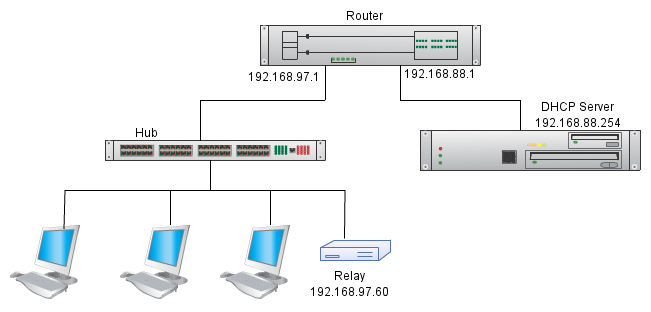
\includegraphics[width = 0.8\textwidth]{Embeddednetwork.png}
\caption{An example topology of a correctly installed relay}
\label{fig:network}
\end{figure}
\section{Documentation for the system engineer}
\label{sec:engineer}
To prepare the relay you just have to flash the relay software on the board. To do this just follow the following steps:
\begin{enumerate}
\item Connect the board and your computer with a router.
\item Open your console.
\item Navigate to the folder project2 which contains the source code.
\item type the following command: \textit{sudo make project2}
\label{itm:command}
\item type: \textit{tftp 192.168.97.60}
\item type: binary
\item type: verbose
\item type: trace
\item Press on the reset button of the board.
\item Wait until the light of the router port on which the board is connected lights up.
\item type: put project2.hex
\end{enumerate}
The relay is now ready for use. To test it you have to install the router as described in \ref{sec:user}. If the pc's are getting an ip from the DHCP server when they do a request, the relay is working correctly.
\section{Documentation for programmers}
The program consists of some initialization functions and one giant switch statement. Every case statement contains a task. So the relay will try to do an action, if it succeeds it goes to the next case otherwise it will retry the current case because the whole switch statement is located in a while lus. This is a list of the tasks in the switch statement in the order they occur in the code:
\begin{enumerate}
\item Set up a connection to listen to breadcasts on the subnet
\item Listen to a DHCP broadcast on the subnet and change the GIADRR field
\item Send an ARP message to get the MAC address of the gateway
\item Receive the ARP response with the MAC address of the gateway
\item Setting up the connection with the DHCP server
\item Transmit the received DHCP packet to the dhcp server through the gateway
\item Setting up a connection to listen to the responses of the DHCP server
\item Listen to a response of the DHCP server
\item Setting up a broadcast connection on the subnet of the relay
\item Broadcast the response in the subnet
\end{enumerate}
\end{document}
